%%
%% This is file `sample-sigconf.tex',
%% generated with the docstrip utility.
%%
%% The original source files were:
%%
%% samples.dtx  (with options: `sigconf')
%% 
%% IMPORTANT NOTICE:
%% 
%% For the copyright see the source file.
%% 
%% Any modified versions of this file must be renamed
%% with new filenames distinct from sample-sigconf.tex.
%% 
%% For distribution of the original source see the terms
%% for copying and modification in the file samples.dtx.
%% 
%% This generated file may be distributed as long as the
%% original source files, as listed above, are part of the
%% same distribution. (The sources need not necessarily be
%% in the same archive or directory.)
%%
%% The first command in your LaTeX source must be the \documentclass command.
%% \documentclass[manuscript,review,anonymous]{acmart}
\documentclass[manuscript, nonacm]{acmart_no_footer}
%% NOTE that a single column version may be required for 
%% submission and peer review. This can be done by changing
%% the \doucmentclass[...]{acmart} in this template to 
%% \documentclass[manuscript,screen]{acmart}
%% 
%% To ensure 100% compatibility, please check the white list of
%% approved LaTeX packages to be used with the Master Article Template at
%% https://www.acm.org/publications/taps/whitelist-of-latex-packages 
%% before creating your document. The white list page provides 
%% information on how to submit additional LaTeX packages for 
%% review and adoption.
%% Fonts used in the template cannot be substituted; margin 
%% adjustments are not allowed.
%%
%%
%% \BibTeX command to typeset BibTeX logo in the docs
\AtBeginDocument{%
  \providecommand\BibTeX{{%
    \normalfont B\kern-0.5em{\scshape i\kern-0.25em b}\kern-0.8em\TeX}}}

%% Rights management information.  This information is sent to you
%% when you complete the rights form.  These commands have SAMPLE
%% values in them; it is your responsibility as an author to replace
%% the commands and values with those provided to you when you
%% complete the rights form.
\setcopyright{acmcopyright}
\copyrightyear{2022}
\acmYear{2022}
\settopmatter{printacmref=false}

%%
%% Submission ID.
%% Use this when submitting an article to a sponsored event. You'll
%% receive a unique submission ID from the organizers
%% of the event, and this ID should be used as the parameter to this command.
%%\acmSubmissionID{123-A56-BU3}

%%
%% The majority of ACM publications use numbered citations and
%% references.  The command \citestyle{authoryear} switches to the
%% "author year" style.
%%
%% If you are preparing content for an event
%% sponsored by ACM SIGGRAPH, you must use the "author year" style of
%% citations and references.
%% Uncommenting
%% the next command will enable that style.
% \citestyle{acmauthoryear}

%%
%% end of the preamble, start of the body of the document source.
\begin{document}

%%
%% The "title" command has an optional parameter,
%% allowing the author to define a "short title" to be used in page headers.
\title{Fret Ferret: Driving Educational Games with Contextual Multi-Armed Bandits to Accelerate Human Learning}

%%
%% The "author" command and its associated commands are used to define
%% the authors and their affiliations.
%% Of note is the shared affiliation of the first two authors, and the
%% "authornote" and "authornotemark" commands
%% used to denote shared contribution to the research.
\author{Douglas Mason}
\email{douglas@koyotescience.com}
\affiliation{%
  \institution{Koyote Science, LLC}
  \streetaddress{}
  \city{San Francisco}
  \state{California}
  \country{USA}
  \postcode{94114}
}

\author{Dan Cote}
\email{dan@koyotescience.com}
\affiliation{%
  \institution{Koyote Science, LLC}
  \streetaddress{}
  \city{San Francisco}
  \state{California}
  \country{USA}
  \postcode{94114}
}
%%
%% By default, the full list of authors will be used in the page
%% headers. Often, this list is too long, and will overlap
%% other information printed in the page headers. This command allows
%% the author to define a more concise list
%% of authors' names for this purpose.
\renewcommand{\shortauthors}{Mason and Cote}

%%
%% The code below is generated by the tool at http://dl.acm.org/ccs.cfm.
%% Please copy and paste the code instead of the example below.
% %%
% \begin{CCSXML}
% <ccs2012>
%   <concept>
%       <concept_id>10010405.10010489.10010491</concept_id>
%       <concept_desc>Applied computing~Interactive learning environments</concept_desc>
%       <concept_significance>500</concept_significance>
%       </concept>
% %   <concept>
% %       <concept_id>10003120.10003123.10010860.10010858</concept_id>
% %       <concept_desc>Human-centered computing~User interface design</concept_desc>
% %       <concept_significance>300</concept_significance>
% %       </concept>
%   <concept>
%       <concept_id>10010147.10010257.10010282.10010292</concept_id>
%       <concept_desc>Computing methodologies~Learning from implicit feedback</concept_desc>
%       <concept_significance>500</concept_significance>
%       </concept>
%   <concept>
%       <concept_id>10010147.10010257.10010282.10011304</concept_id>
%       <concept_desc>Computing methodologies~Active learning settings</concept_desc>
%       <concept_significance>500</concept_significance>
%       </concept>
%  </ccs2012>

% \end{CCSXML}

% \ccsdesc[500]{Applied computing~Interactive learning environments}
% % \ccsdesc[300]{Human-centered computing~User interface design}
% \ccsdesc[500]{Computing methodologies~Learning from implicit feedback}
% \ccsdesc[500]{Computing methodologies~Active learning settings}
% % %%
% % %% Keywords. The author(s) should pick words that accurately describe
% % %% the work being presented. Separate the keywords with commas.
% \keywords{machine learning, bandit algorithms, interface design}

%% A "teaser" image appears between the author and affiliation
%% information and the body of the document, and typically spans the
%% page.
% \begin{teaserfigure}
%   \includegraphics[width=\textwidth]{canonical_image_fret_ferret.png}
%   \caption{Example user interface for identifying intervals visually on the guitar fretboard, with the questions determined by a contextual multi-armed bandit aiming for moderate-to-high difficulty and that has been partially trained.}
%   \Description{Computer interface with one range selector for input}
%   \label{fig:teaser}
% \end{teaserfigure}


\begin{abstract}
\\
This work introduces the world's most robust software trainer for the guitar, called \textit{Fret Ferret}, which utilizes the contextual multi-armed bandit class of algorithms, as well as implicit signals from the user, to customize lessons to each user automatically and in real time, avoiding the need to tweak a large selection of game parameters in order to obtain a desired difficulty level. We discuss the consequences of using these algorithms to drive new styles of computer-human interaction that can accelerate our learning process and help us reach new mental achievements. We elaborate on the details of our algorithms, how they inform our user interface design, and how we address the difficulty of scaling the development of a large number of machine learning models to adapt to many mini games and each user individually. Finally, we address future work that can further augment the performance and capabilities of our software.
\end{abstract}

%%
%% This command processes the author and affiliation and title
%% information and builds the first part of the formatted document.
\maketitle


\begin{figure}[h]
  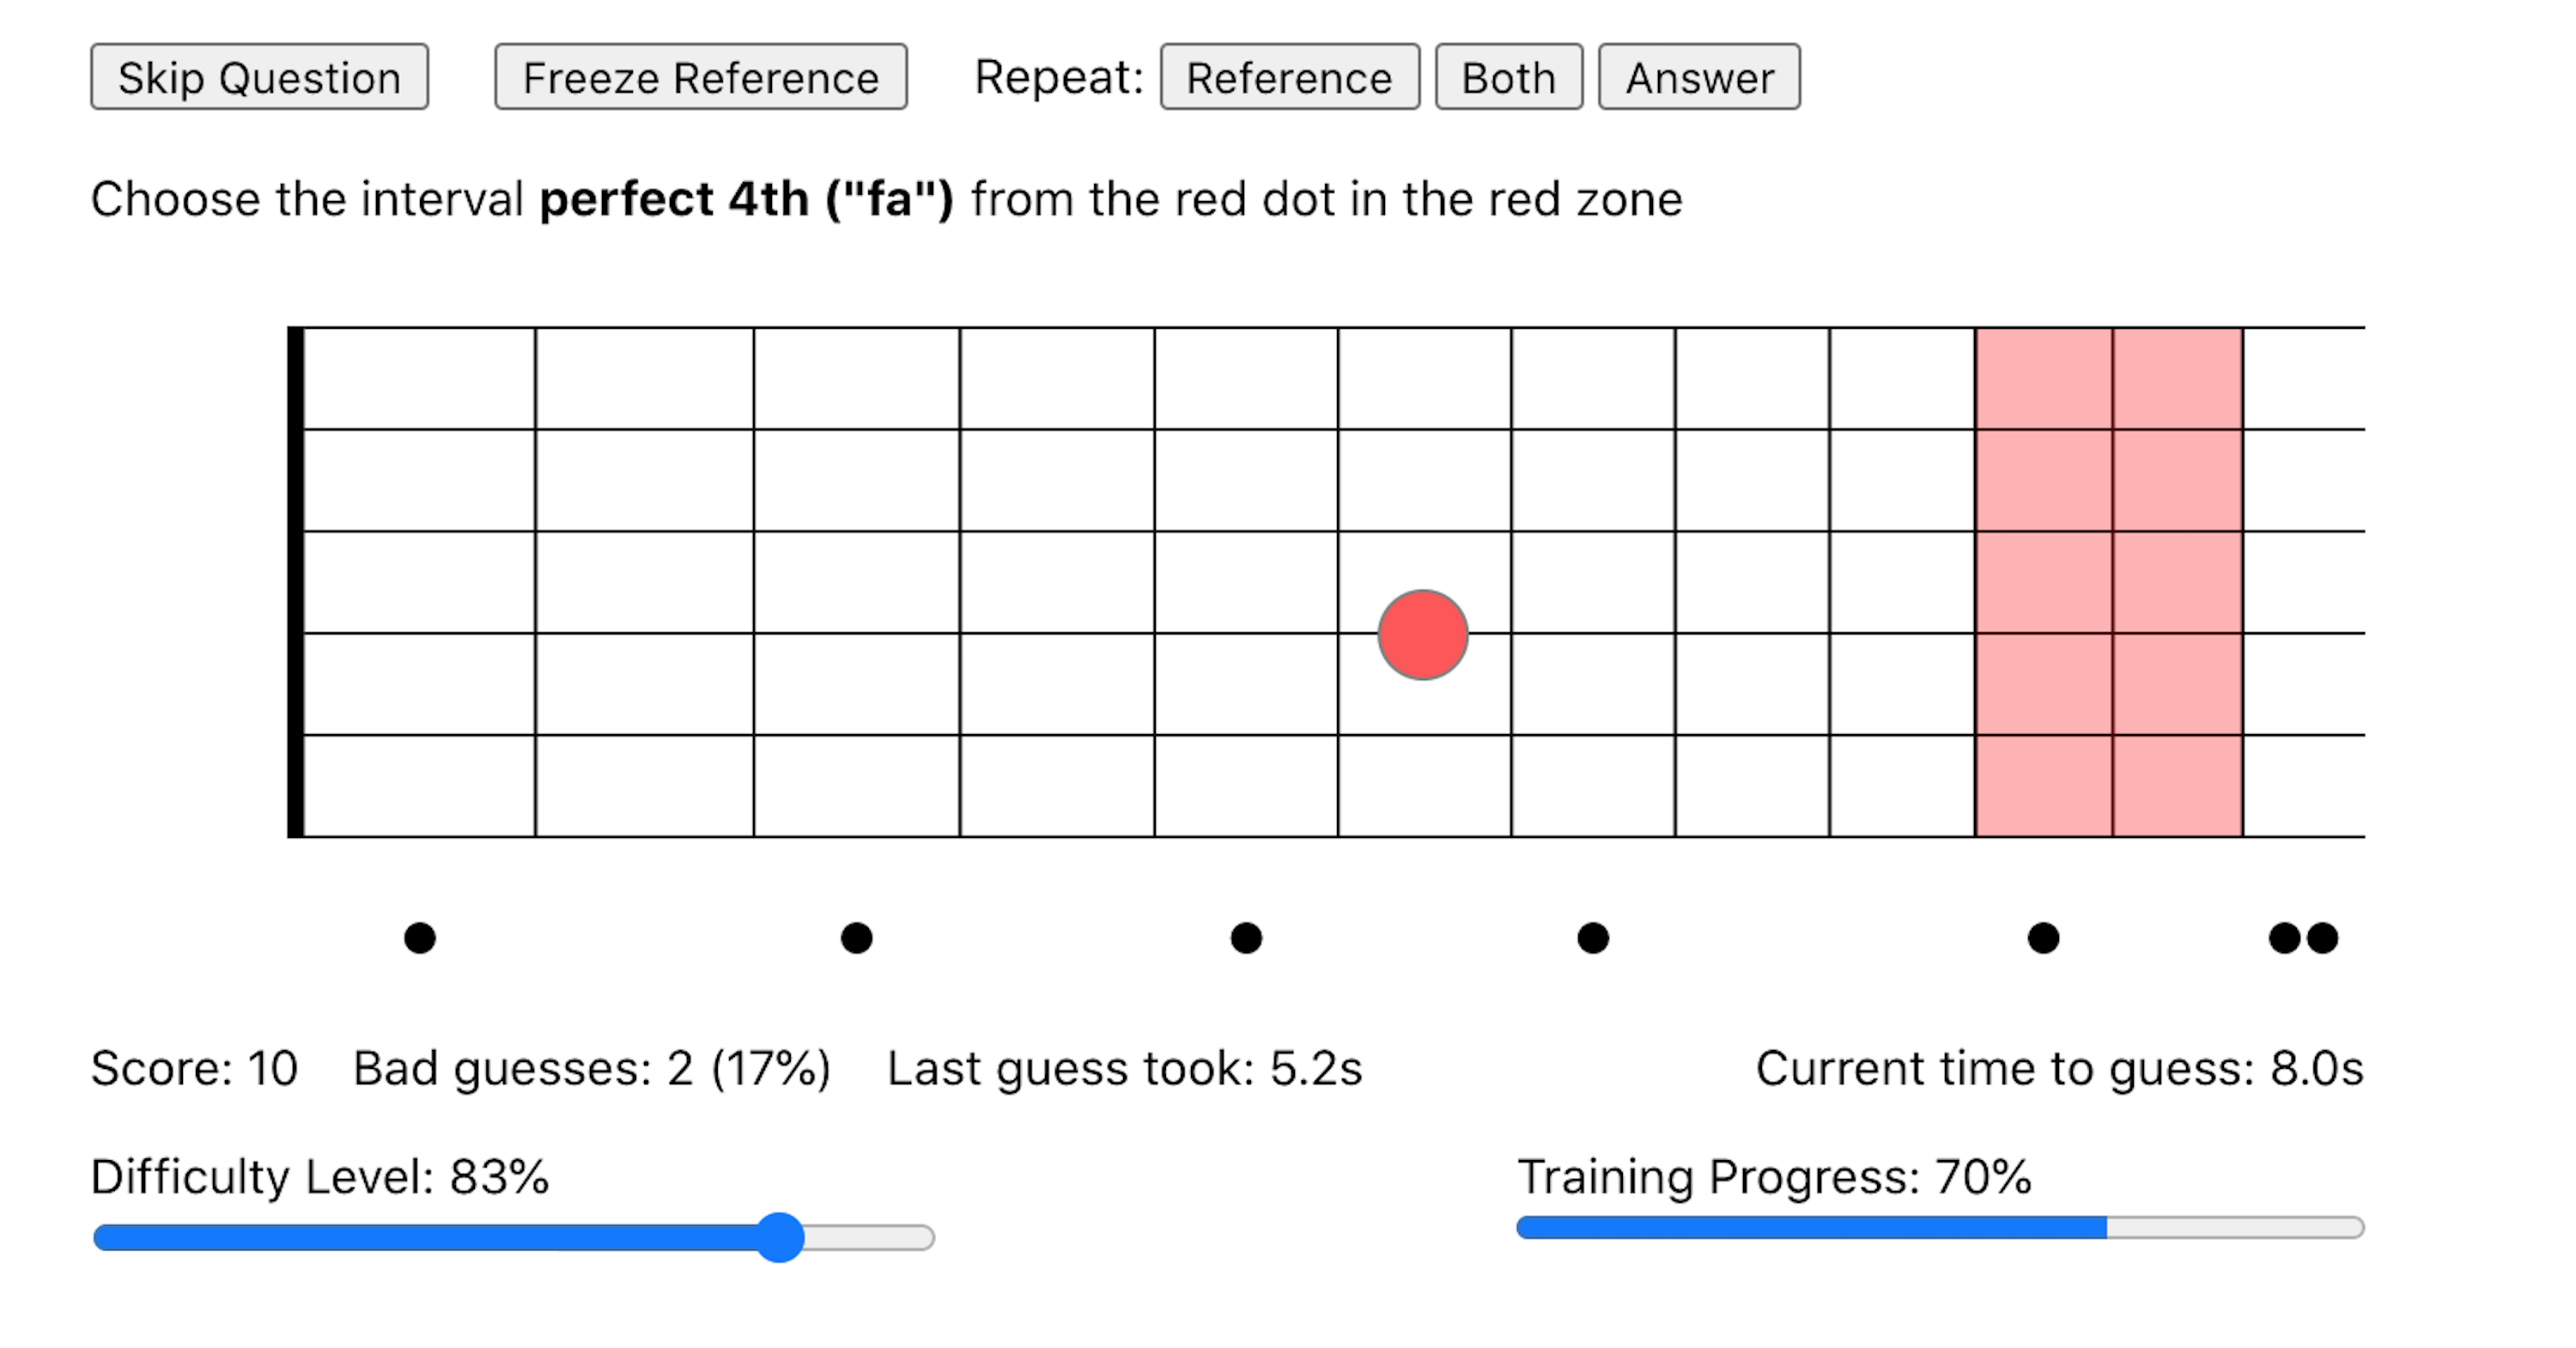
\includegraphics[width=\linewidth]{canonical_image_fret_ferret copy.png}
  \caption{Example user interface for identifying intervals visually on the guitar fretboard, with the questions determined by a contextual multi-armed bandit aiming for moderate-to-high difficulty and that has been partially trained.}
  \Description{Computer interface with one range selector for input}
  \label{fig:teaser}
\end{figure}

\section{Introduction}

Software for training guitar players has generally been limited to random selections of questions with a focus on correctness over speed\cite{guitar_trainer1, guitar_trainer2, guitar_trainer3}.  However, users quickly get bored when such systems ask too many questions they know by heart, or ask questions that are outside of their abilities. To address this limitation, the common solution has been to offer a large variety of randomization parameters for the user to adjust in order to eliminate questions as they become easier to answer. 

Here we introduce our own guitar training software \textit{Fret Ferret} to show how we have marshaled a contextual multi-armed bandit algorithm\cite{multi_armed_bandits1, multi_armed_bandits2} to quickly learn from implicit user feedback during early trials. This allows us to hide the randomization parameters and automatically alter question selection to optimize for a desired difficulty level. For example, if a user desires high difficulty, the system will select questions which are likely to take the longest to answer and focus on their weak spots. If this proves too challenging to stay enjoyable, the user can reduce the difficulty by adjusting one intuitive parameter rather than many confusing ones (see Figures 1 \& 2).

The multi-armed bandit class of algorithms\cite{multi_armed_bandits1, multi_armed_bandits2} were first introduced in the 1980s, but only recently have technological developments and improved methods allowed us to implement them easily and cheaply. In the last decade, they have exploded onto the education research scene\cite{bandits_education_survey, bandits_education_axis, bandits_education_clement1, bandits_education_liu, bandits_education} as an ideal method for automatically tailoring questions to students without human intervention, which can greatly reduce labor costs and increase access. While bandits optimize for an immediate response, such as correctness or speed of the question at hand, reinforcement learning algorithms additionally consider how sequences of decisions can lead to longer-term responses over multiple questions, such as how long the student continues to use the system, which have also been explored in the literature\cite{rl_education_survey, rl_education_nips, rl_education_amazon}. Similarly, multi-armed bandits\cite{bandits_interface, bandits_games} and reinforcement learning\cite{rl_game, rl_game2} have been explored for game and interface design, among many other applications\cite{bandits_applications, rl_applications}.

Beyond the literature we have examined on multi-armed bandit and reinforcement learning applications in educational games, this article contributes the following: 
\begin{itemize}
\item Our reward signal is based on \textbf{time-to-completion} instead of answer correctness.
\item We \textbf{enhance exploration} using intuitive parameters that designers and users can adjust during gameplay.
\item We address the challenge of \textbf{feature engineering} and hyperparameter tuning in an online fashion that is inconspicuous to the user and requires no manual oversight.
\item We combine state-of-the-art algorithms with \textbf{multiple modes of interactions} for a comprehensive educational experience
\end{itemize}
All of these contributions have been born out of necessity for building a large corpus of auto-personalizing games quickly which can respond to the unique needs of advanced musical education. 

Moreover, in this article we will discuss how merging multi-armed bandits with novel interaction mechanisms presents unique challenges for interface and machine learning model design, with each informing the other. For example, the bias-variance trade-off\cite{bishop} in machine learning manifests itself by determining how long it takes for a game to correctly predict the difficulty of each question for the user, making model tuning critical to finding the right balance. This challenge arises because we are focused on building personalized curricula, rather than optimizing one curriculum over multiple students. We discuss our solution, which we call \textit{HyperTune}, and which makes it easy to deploy the most enjoyable, effective educational tool possible with the latest advances in machine learning.

\section{Why Use Multi-Armed Bandits?}

Multi-armed bandits are commonly used in commercial technology to optimize websites\cite{bandit_website_optimization} as a replacement for A/B testing of different presentation options, such as choosing between two headlines for a newspaper article\cite{new_york_times_headlines}. These algorithms automatically navigate the exploration/exploitation trade-off by first selecting options randomly (exploration) then honing in on the most promising ones (exploitation) in a manner that reduces the regret (the difference between real-world performance and ideal performance). Because of their data efficiency, bandits are ideal for personalization in situations where there are few opportunities to learn a user's preferences.

In our application, we use a multi-armed bandit to optimize for a desired difficulty level as evaluated implicitly by time-to-completion: high difficulty correlates to questions that take the longest to answer, and vice versa. Difficulty is measured as the percentile of random questions whose predicted time-to-completion are shorter than the measured time-to-completion for the given question. The bandit trains against the time-to-completion target, and questions are ranked according to the rank score. Given a prescribed difficulty level $D$, question $Q$ with predicted time-to-completion $T(Q)$, and time-to-completion percentile $P(Q;\mathcal{Q})$ for $Q$ among all questions $\mathcal{Q}$, we write the rank score as \begin{equation}\label{eq:rank_score}R(Q)=\text{abs}\left[P(Q;\mathcal{Q})-D\right]\end{equation}Ranking is unaffected by additive shifts or multiplicative constants. Note that because of the additional restraint of matching a desired difficulty level, our approach does not match the bandit formalism strictly, except when $D$ is set to 100\%. Rather, we have decoupled the target that the bandits are trained against from the ranking procedure used to select questions, but the desired behavior remains the same.

We chose time-to-completion as a metric for many reasons, beginning with the fact that it is very difficult to cheat, making it one of the most reliable measures of cognition in the psychology literature, as highlighted by the Implicit Association Test\cite{implicit_association_test}. Another benefit is that our target audience of musicians desire not only to be correct, but to recall information as quickly as possible. Moreover, optimizing computer-human interaction to consistently operate at the edge of the user's abilities is the hallmark of creating "flow" states that are intrinsically enjoyable to the user and critical for creative development\cite{flow}, while keeping users engaged and excited to keep using our system. Without automated difficulty matching, users are forced to answer many questions that are beneath or above their level, which becomes boring or frustrating, leading to churn.

\section{Strategy Considerations}

Bandits are necessary in environments where data is expensive to collect -- in our case, because each question requires time for the user to respond, and because users have limited patience. When a bandit makes predictions and acts on them with a given strategy, it not only samples the most promising options, it also learns the most about the domain of data where those options reside. Unlike traditional supervised machine learning models, which attempt to reflect the full domain of possible inputs in an unbiased fashion, bandits are intentionally blind to unexplored regions in the input space since it is costly to obtain information about them. In our application, this behavior manifests itself when the user changes the desired difficulty level, since the bandit must re-engage exploration, and will make some wrong guesses as it learns about the new data domain, until it is confident it can exploit at the new difficulty level again.

There are many strategies available to automate this process, chief among them are (1) the "epsilon-greedy" strategy\cite{bandit_website_optimization}, which only uses a prediction model for selecting options for a given fraction of questions, usually around 80\%, and selects randomly otherwise, (2) the Upper Confidence Bound (UCB) strategy\cite{UCB}, which ranks options based on their predicted outcomes in addition to their uncertainties, and (3) Thompson sampling\cite{thompson_sampling1, thompson_sampling2, bootstrap_facebook}, in which the prediction model is replaced by a distribution of models, one of which is sampled to perform predictions for each question that is asked. Model predictions, and their confidence intervals, are transformed by Equation \ref{eq:rank_score} before being acted upon any given strategy. For our application, we use Thompson sampling because it only introduces one hyperparameter to tune, the number of prediction samples, which is generally set to 100, and it has shown stronger performance over epsilon-greedy and UCB in similar contexts\cite{thompson_sampling3}. 

For the prediction model, we use a custom implementation of Bayesian linear regression\cite{BLR, Mason_Gaussian_processes_and_2021} (BLR), which provides us model distributions and Bayesian sampling to enable Thompson sampling. BLR has the benefit of only requiring $\mathcal{O}\left(N_\text{features}^2\right)$ storage and $\mathcal{O}\left(N_\text{features}^3\right)$ computation, where $N_\text{features}$ is the number of features in the model. Unlike other models like Gaussian processes or nearest neighbors regression, the computational and storage costs BLR does not scale with the amount of data it has been trained on, thus making it an incremental, online, or streaming algorithm with good performance guarantees. Moreover, because BLR is a convex optimization problem, it is always guaranteed to converge regardless of our hyperparameters, unlike stochastic gradient descent and neural networks that are popular in deep learning but which can get stuck in local extrema in their optimization landscape, requiring extensive hyperparameter tuning. BLR is also wildly more efficient for prediction than random forests, which is critical for latency-sensitive tasks like interactive games. Most importantly, these properties allow BLR to introduce only one new hyperparameter to tune: the regularization constant, which can generally be left to a standard value such as 1/100th of the vector norm of the inputs after a set number of inputs have been observed.

With \textit{Fret Ferret}, users specify a difficulty level between 0\% and 100\%, with the default set to 80\%, and which is interpreted as a difficulty percentile of available questions. We found that only choosing the question at that exact percentile, which is the traditional bandit setup, led to poor experiences with insufficient variety to keep the user engaged, even though Thompson sampling partially randomizes its selection process anyways. Thus, we artificially increased the variety of our question by selecting not only the most-closely-ranked question, but also others selected at random from a 10\% population pool of questions with ranks close to the desired percentile. Anecdotal evaluations found this approach to be much more enjoyable and led to longer sessions. 

\section{Using \textit{HyperTune} to Scale Model Development Over Many Games}

The guitar trainer software we designed is a collection of many mini-games, each requiring a different prediction model to run its associated multi-armed bandit. The list of available games comes from the cross product of key skills we aim to train. On the one hand, players must be able to locate notes which are provided by name to gain a good \textit{absolute} understanding of the fretboard, as well as musical intervals which can be written or played musically to gain a good \textit{relative} understanding. On the other hand, we force users outside of their comfort zone by asking them to identify these locations under various restrictions which mimic common playing situations: (1) anywhere on the fretboard, (2) on a specified string, or (3) within a specified region of contiguous frets, usually 3 but other sizes are possible. Higher-level games include spelling out all notes in a chord or scale, starting with either a root name or location indicated visually on the fretboard. At the highest level, a chord progression can be performed by our web app, with the corresponding notes shown on the app's fretboard, while the performer improvises their own melodies which are also visually indicated on the same fretboard, to identify when the performer is playing "within" the chord and when they are playing "outside". The chord progressions can be defined by the user and even include key changes, making this interaction mode ideal for developing jazz fluency.

We have provided a syllabus of 32 such games in increasing order of sophistication to help the user along their journey.  While this breadth enables us to work with players possessing a wide range of education levels, the large number of mini games introduces the burden of engineering the features used to train the models that run the bandits powering each game. Notably, as more features are added -- for example, not only encoding which fret the answer note is played on, but also the string -- the model begins with greater uncertainty in its predictions, requiring more trials before it can refine those uncertainties. The bias-variance trade-off expresses itself in our games such that models with more features are more capable of finding diamonds in the rough, such as a particularly challenging fretboard location or note name for the user. Conversely, models with fewer features quickly pick out gestalt features, such as which strings or fretboard areas the user has difficulty with, but are incapable of refining their predictions further. Early efforts tuned the feature sets through trial-and-error to find those that allow the model to learn as quickly as possible while still capturing the most important aspects for predicting difficulty. 

However, feature engineering is arduous and prone to error, making such systems difficult to scale or for new developers to utilize. Moreover, the best feature engineering for a given game may be specific to each user. For this reason, we incorporate the \textit{HyperTune} system into our model, by which the developer can specify $M$ sets of model parameters, which include parameters for the feature engineering used, that the system may consider. For each parameter set, $N$ copies of the model are trained on a different sampling of $\frac{\max(N, 5)-1}{\max(N, 5)}$ of the full dataset, with the remaining $\frac{1}{\max(N, 5)}$ of data held out for validation and stored. We apply the max operator $\max(N, 5)$ to ensure that at most 20\% of data is reserved for validation. $N$-fold cross-validation is performed at regular intervals for each parameter set, whereby the associated model's performance over the validation data is averaged over the $N$ copies. The set with the best average performance is selected, and an associated model that has been trained on all the data is silently deployed to the user. 

This setup allows us to perform \textit{HyperTune} in a streaming manner, with training latency and storage increased only by the constant factor $N\times M$,  where $N=1$ is often sufficient. However, the user only experiences the inference latency period, which is unaffected by \textit{HyperTune}, so that they are oblivious to the work happening behind the scenes serving them the best possible model available. In addition, by using a reservoir sampler\cite{reservoir_sampler} to store the validation data, we can impose an upper limit on storage costs while maintaining an accurate representation of the data that has been seen.

Because the data we use to train our models is biased towards questions favored by the bandit that collected the data, it is helpful to compensate for this bias using \textit{inverse probability weighting}\cite{ipw}. In this approach, the probability that the currently-engaged bandit selected a given question indexed by $i$ is written as $\pi_{i}$, and we weight the data used to train all our models by $\text{IPW}_i=\frac{1}{\pi_{i}}$. This ensures that feedback for questions which had a low likelihood being selected have a larger impact on subsequent decisions. Because of the inverse proportionality, numerical instabilities can arise when actions are given very small probabilities, but this is ameliorated by adding artificial exploration through an epsilon-greedy policy or other strategies, such as selecting questions from a ranked pool. Further elaboration, called \textit{augmented inverse probability weighing} or \textit{doubly-robust estimation} can also be considered\cite{doubly_robust_estimators}.

Without \textit{HyperTune}, a single model can be measured in terms of "progress", a term indicating how many varied samples have been encountered that lead to confident predictions of question difficulty. How this value is determined is left up to the developer, and is subjective in nature. For \textit{Fret Ferret}, we define 100\% progress as having seen at least 5 examples featuring each possible feature value for categorical variables, such as 5 examples for each string and 5 examples for each fret. Additional measures can be made for continuous variables, for example, by using domain knowledge to bin inputs to create equivalent categorical variables. 

Employing \textit{HyperTune} means that our models are continuously trained and swapped as they learn, so that like a car shifting to higher gears, the progress presented to the user drops down briefly as the more feature-rich is swapped in. However, we found that users respond better to a monotonically increasing measure of training progress as a goal to reach, and that simple heuristic measures like the one proposed here were more predictable and rewarding than direct measure of prediction uncertainty which can fluctuate substantially. For our user interface, we kept the progress bar for the hand-tuned feature engineering we found worked well in general, but future measures of progress may be explored that are more consistent with the underlying models being used. 

\begin{figure}[h]
  \centering
  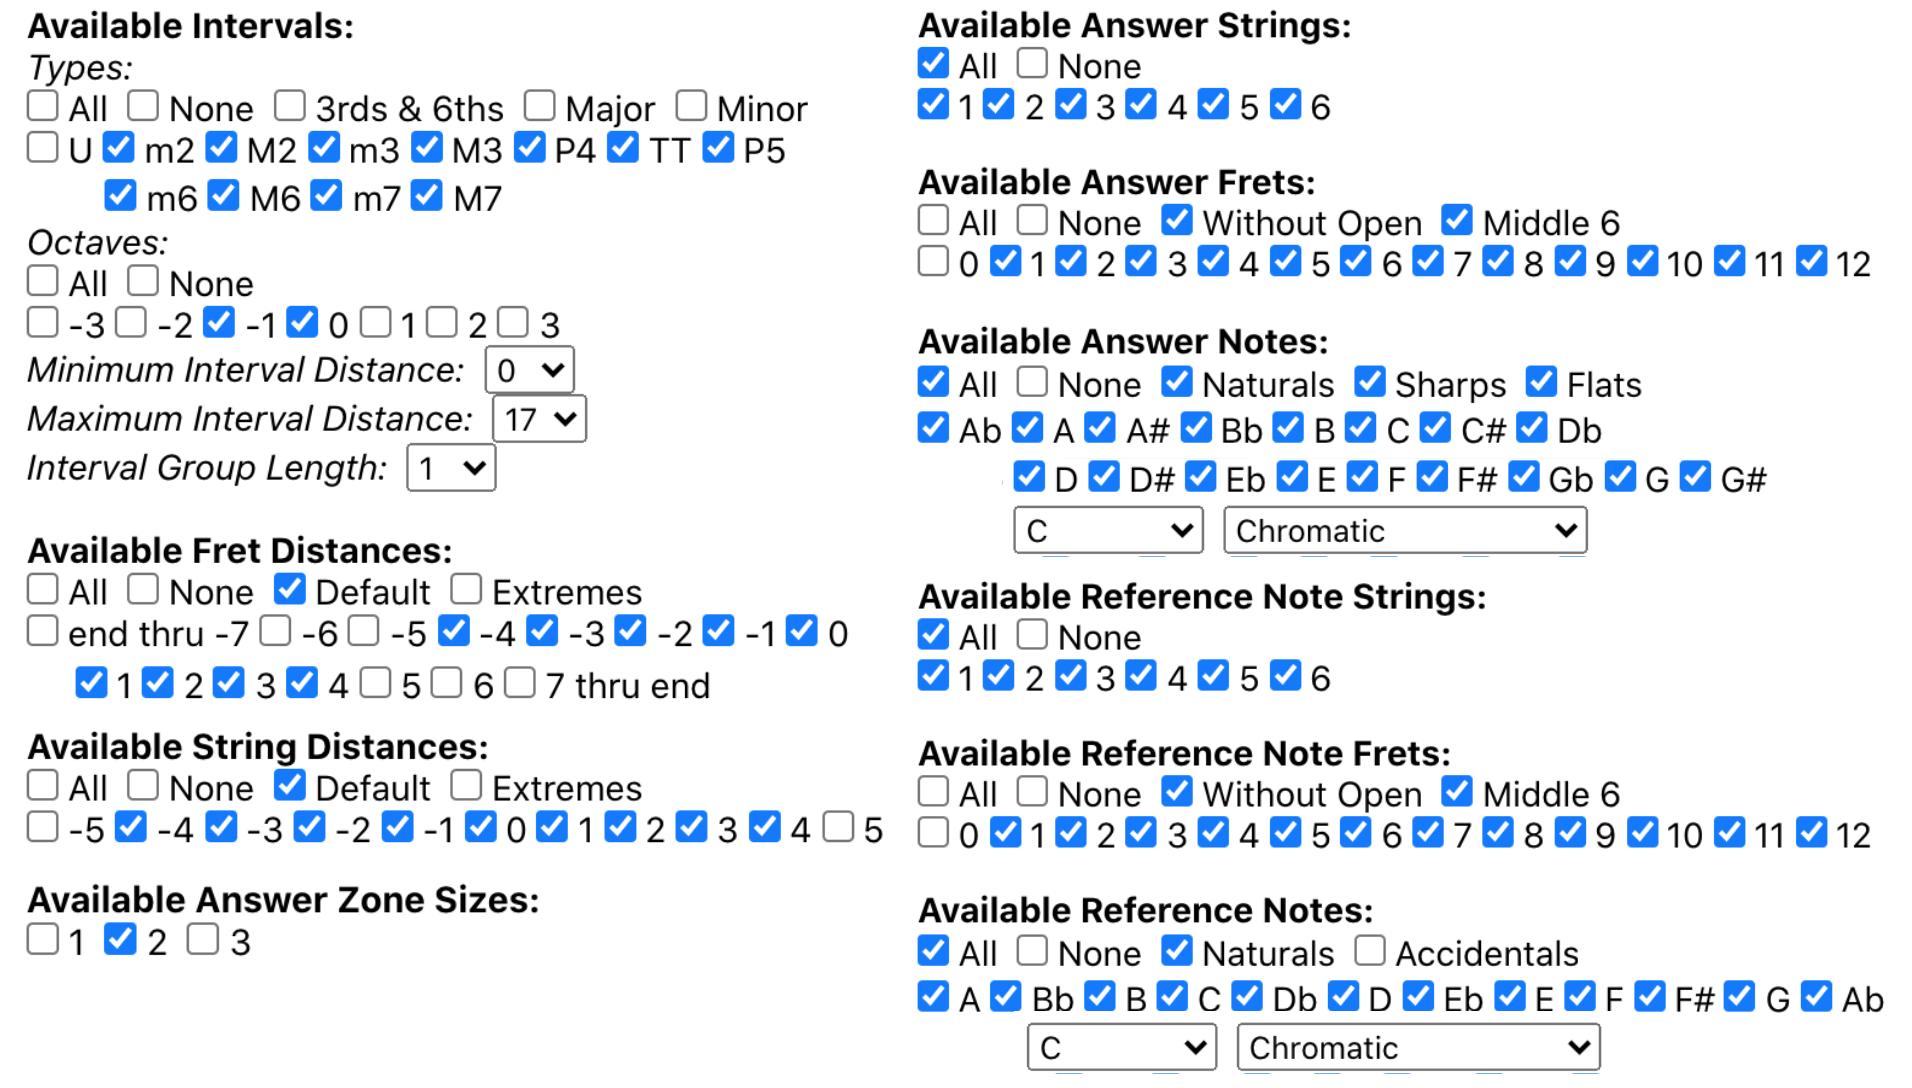
\includegraphics[width=\linewidth]{list_of_randomization_settings.png}
  \caption{The randomization parameters users otherwise need to adjust for the game in Figure 1. This image is taken from actual gameplay and was the original approach used before the algorithms in this article were implemented.}
  \Description{Computer interface with hundreds of labels and check boxes}
  \label{fig:randomization_parameters}
\end{figure}

\section{Modes of Interaction}

Working with the field of music provides a wide variety of ways to interact with software, in part thanks to the proliferation of portable touch-screen devices with high-quality speakers and microphones that can even work simultaneously without overstepping each other. At the moment, \textit{Fret Ferret} provides the following avenues for interacting with the software:
\begin{itemize}
\item The user can click with a mouse or their finger on the fret position and string corresponding to their answer
\item The user can play the corresponding note, either on their own guitar or any instrument of their choosing, even by humming the note
\item The user can play the corresponding note on a MIDI instrument connected to the device
\end{itemize} While working directly with the GUI is intuitive and always-available, the last two modes open up exciting possibilities with ear-training and transferring knowledge directly to the instrument, since the user can work with their native instrument instead of mapping one's knowledge to a GUI. These modes also make \textit{Fret Ferret} a viable trainer for any instrument, but without the added restrictions of forcing the user to play notes on a given string or fret region which are specific to the guitar. 

With modern pitch detection software\cite{pitchfinder}, accurate predictions of pitch can be made within a few hundred milliseconds. This means that while fast solos and runs are difficult to accommodate, moderate speed and rhythm can be maintained throughout the training session. Combining pitch detection with audio cues, an entirely-audio game can be played. Users of \textit{Fret Ferret} that have worked with this mode have reported not just improved abilities at the guitar, but also improved listening skills that help the user identify the scale degrees (the "do-re-mi" label) of music that they listen to in real-time, helping them become better composers and improvisers.

A single note, such as E, can be played in many places on the guitar. Audio- and MIDI-based interaction modes are unable to pick up on the specific fret position or string that the user played. However, such interactions could be facilitated by an electronic instrument that delineates those distinctions\cite{guitar_trainer_physical}, or by machine learning models that specialize in interpreting audio and/or video signals for this purpose. More experimental solutions include using models to predict the most likely location where the user played the note, which has been explored in automated tablature transcriptions\cite{guitar_DL1} and predicting the location of mouse clicks using long-short-term memory models\cite{predict_mouse_click}. For our purposes, however, such elaborations have been unnecessary because there are few reachable notes from a given position, and the likelihood of choosing the same note outside of the restrictions is low (1/12 or 8\%). Moreover, this error has little impact on the sound that is actually produced. While pitch detection for single notes is a mostly-solved problem with many viable alternatives\cite{pitchfinder} ready to be used, pitch detection for multiple notes at once is an ongoing field of research\cite{polyphone_pitch_detection}, and could be used in the future to add chord-playing without the requirement to hit each note individually.

\section{Conclusions and Future Work}

The \textit{Fret Ferret} guitar training software introduced here is unique for using implicit feedback and machine learning to tune its questions to the user automatically, radically simplifying the interface design so that only a single parameter needs to be controlled. This allows for easy adoption and a comfortable learning experience that eliminates wasted time as the student reaches towards their goals. Incorporating the \textit{HyperTune} system, and being aware of the various impacts that our algorithm design have on the user experience, have allowed \textit{Fret Ferret} to far exceed our expectations. By demonstrating the system and identifying key stumbling blocks, we hope to encourage others to create more educational tools driven by artificial intelligence that improve our human intelligence. There are, however, many ways we hope to improve our system and \textit{Fret Ferret} further.

One limitation to the bandit framework is that it treats every question on its own without considering how sequences of questions can lead to harder or easier experiences for the user. For example, if a question is repeated, it will likely be a lot easier the second time around. One general solution to this problem is to add historical data to the feature set, such as providing the same features used to for the current question in order to describe previous questions in the queue. The most general solution may also add possible interactions between the same features for the different questions, such as whether the previous questions featured the same strings or frets. A major drawback to this class of solutions, however, is that models trained with such large feature sets fail to learn quickly and impose higher resource overhead in every aspect of computation. Alternatively, heuristics can be used to filter out question from the ranking pool, such as those which were recently asked, which is used in \textit{Fret Ferret}. However, the most principled approach to handling sequential planning is to use the full force of reinforcement learning.

The most natural extension from bandits into the broader tool set of reinforcement learning is to graduate from bandits to $Q$-learning\cite{sutton_barto_rl} by training against not just the immediate signal (time-to-answer for the given question), but an aggregate of future rewards signals, such as the average time it takes the user to answer the following $N$ questions, or the maximum time to answer a question within that set. Similarly to inverse probability weighting, we also must adjust these rewards using importance sampling in the Thompson-sampling setting, as discussed in Section 4.3,  "The connection between multi-armed bandits and $Q$-learning" in \cite{Mason_Real-World_Reinforcement_Learning_2021}. Further development may work with the policies themselves in an approach known as \textit{policy optimization}\cite{online_policy_gradient_review}. We hope to explore all these possibilities in the near future.

\textit{Fret Ferret} is run by federations of models in the \textit{HyperTune} system, whereby each federation is unique to each mini game and user, and therefore its models start from scratch whenever they encounter a new user or a user begins a new game. This arises because we are focused on building personalized curricula, rather than optimizing one curriculum over multiple students, although the algorithms discussed here can be easily adapted to either setting. However, this limitation poses the question: What if we could address both optimization problems simultaneously? 

Merging global with personal optimization is a broad goal of the recommender systems and automated personalization literature\cite{recsys_applications, recsys_survey_deep_learning}, which has also explored incorporating multi-armed bandit and reinforcement learning algorithms\cite{rl_recsys, rl_recsys2, rl_recsys3}. We have considered a few approaches for future development. One trains a global federation of models for all users and each mini game, then creates a copy of each global model to fine-tune it to each user, in a process called transfer learning\cite{transfer_learning, transfer_learning2}. Another uses predictions from the global model as an additional input to an associated personalized model, allowing the personalized model to learn a gate parameter that determines how much to weigh the contribution from the global model\cite{mason_bandtis_recsys}. Because the gate parameter is interpretable, it gives the developer or user control over the influence of global predictions even as the bandit learns the ideal value. This control can be introduced through the use of prior beliefs or by direct manipulation, with the drawback that the cumulative reward may not be maximized. 

Lastly, the interactive demonstration presented here has not been subjected to user experience studies, by which we can measure user progress and retention as a function of the parameters we use to define our system, such as the impact of \textit{HyperTune}, using different feature engineering approaches, etc., and we would like to pursue this angle as resources allow. In the meantime, \textit{Fret Ferret} is free and open to the public, along with our 32-course syllabus, and can be accessed at \url{http://fretferret.com}.


%%
%% The acknowledgments section is defined using the "acks" environment
%% (and NOT an unnumbered section). This ensures the proper
%% identification of the section in the article metadata, and the
%% consistent spelling of the heading.
%%\begin{acks}
%%To Robert, for the bagels and explaining CMYK and color spaces.
%%\end{acks}

%%
%% The next two lines define the bibliography style to be used, and
%% the bibliography file.
\bibliographystyle{ACM-Reference-Format}
\bibliography{sample-base}


\end{document}
\endinput
%%
%% End of file `sample-sigconf.tex'.
